% !TeX program = xelatex
\documentclass[12pt,a4paper]{ctexart}
\usepackage{geometry}
\geometry{left=2.5cm,right=2.5cm,top=2.5cm,bottom=2.5cm}
\usepackage{fancyhdr}
\usepackage{graphicx}
\usepackage{amsmath}
\usepackage{float}
\usepackage{caption}
\captionsetup{font=small,labelfont=bf}
\usepackage[hidelinks]{hyperref}
\usepackage{listings}
\usepackage{xcolor}
\usepackage{booktabs}

% 消除 fancyhdr 警告
\setlength{\headheight}{13.6pt}

% ---------- 代码块样式 ----------
\lstset{
    basicstyle=\ttfamily\small,
    keywordstyle=\color{blue},
    commentstyle=\color{gray},
    stringstyle=\color{red},
    showstringspaces=false,
    breaklines=true,
    frame=single,
    backgroundcolor=\color{gray!10},
    numbers=left,
    numberstyle=\tiny\color{gray},
    tabsize=4,
    xleftmargin=2em,
    xrightmargin=2em,
}

% ---------- 中文设置 ----------
\setCJKmainfont{Noto Serif CJK SC}
\setCJKsansfont{Noto Sans CJK SC}
\setCJKmonofont{Noto Sans Mono CJK SC}

% ---------- 页眉页脚 ----------
\pagestyle{fancy}
\fancyhf{}
\fancyhead[C]{\small 系统开发工具基础 · 实验报告（第三周）}
\fancyfoot[C]{\thepage}
\renewcommand{\headrulewidth}{0.4pt}
\renewcommand{\footrulewidth}{0pt}

% ---------- 标题格式 ----------
\usepackage{titlesec}
\titleformat{\section}{\Large\bfseries\centering}{第\thesection 题}{1em}{}
\titleformat{\subsection}{\normalsize\bfseries}{\arabic{subsection}}{1em}{}
\renewcommand{\baselinestretch}{1.3}

\begin{document}

% ==================== 封面 ====================
\begin{center}
    {\Huge\bfseries 系统开发工具基础} \\[0.5cm]
    {\LARGE 每周课上实验报告} \\[0.8cm]
    {\large 第三周（2026年9月7日）} \\[2cm]
    \large
    \begin{tabular}{rl}
        姓\qquad 名： & 李永锋 \\[0.3cm]
        学\qquad 号： & 25030021039 \\[0.3cm]
        实验日期：     & 2026年9月7日
    \end{tabular} \\[2cm]
    \today
\end{center}
\newpage

% ==================== 实验概况 ====================
\section*{实验概况}
\addcontentsline{toc}{section}{实验概况}

本次实验为第三周的四道课上练习题，涵盖 Python 打包与分发（Wheel 构建）、智能体辅助测试驱动修复、协作材料重写（Issue/Commit/Review）以及 PyTorch 深度学习基础（线性回归训练）。通过动手实践，巩固了项目打包流程、测试驱动开发、专业沟通规范以及深度学习框架的基本使用。

\subsection*{实验环境}
\begin{itemize}
    \item 操作系统：Windows 11 + WSL2 (Debian)
    \item Shell：bash 5.0
    \item Python 版本：3.13.5
    \item 已安装工具：Git、python3、pip、pytest、ruff、build、torch（2.13.0）
    \item LaTeX 引擎：XeLaTeX
\end{itemize}

\subsection*{遇到的主要问题与解决}
\begin{enumerate}
    \item \textbf{pyproject.toml 中项目名含中文字符}：`name = "greetlab-学号"` 违反 PEP 508 规范，改为数字学号 \texttt{greetlab-25030021039} 后构建成功。
    \item \textbf{可编辑安装（\texttt{pip install -e .}）后无法导入包}：setuptools 未正确识别 \texttt{src/} 布局，通过设置 \texttt{PYTHONPATH} 临时解决，后续改用显式包配置 \texttt{[tool.setuptools] packages = ["greetlab"]}。
    \item \textbf{虚拟环境隔离导致 PyTorch 缺失}：在 q12 新建独立虚拟环境 \texttt{.venv12} 后安装 torch，解决了跨环境污染问题。
    \item \textbf{Pytest 测试导入失败}：因包未安装或 \texttt{PYTHONPATH} 未设置，最终采用 \texttt{export PYTHONPATH=\$(pwd)/src} 使测试通过。
\end{enumerate}

\newpage

% ==================== 第9题 ====================
\section{从源码构建并在干净环境安装 Wheel}

\subsection{任务目标}
创建一个最小 Python 命令行包，使用 \texttt{build} 工具构建 Wheel，并在全新虚拟环境中安装验证。

\subsection{操作步骤}
\begin{enumerate}
    \item 创建项目目录 \texttt{src/greetlab/}，编写 \texttt{\_\_init\_\_.py} 和 \texttt{cli.py}（含 \texttt{main()} 函数）。
    \item 编写 \texttt{pyproject.toml}，定义构建系统、项目元数据和脚本入口。
    \item 修正项目名中的中文字符，使用数字学号 \texttt{greetlab-25030021039}。
    \item 在虚拟环境中安装 \texttt{build}，执行 \texttt{python3 -m build --wheel} 生成 \texttt{.whl} 文件。
    \item 切换到新目录创建干净虚拟环境，用 \texttt{pip install} 安装 Wheel，运行 \texttt{sdt-greet --name 25030021039} 验证。
\end{enumerate}

\subsection{关键命令与输出}
\begin{lstlisting}[language=bash]
# 构建 Wheel
python3 -m build --wheel
Successfully built greetlab_25030021039-0.1.0-py3-none-any.whl

# 安装并验证
pip install ~/expriment_reports/report_3/q09/dist/greetlab_25030021039-0.1.0-py3-none-any.whl
sdt-greet --name 25030021039
Hello, 25030021039!
\end{lstlisting}

\subsection{演示截图}
\begin{figure}[H]
    \centering
    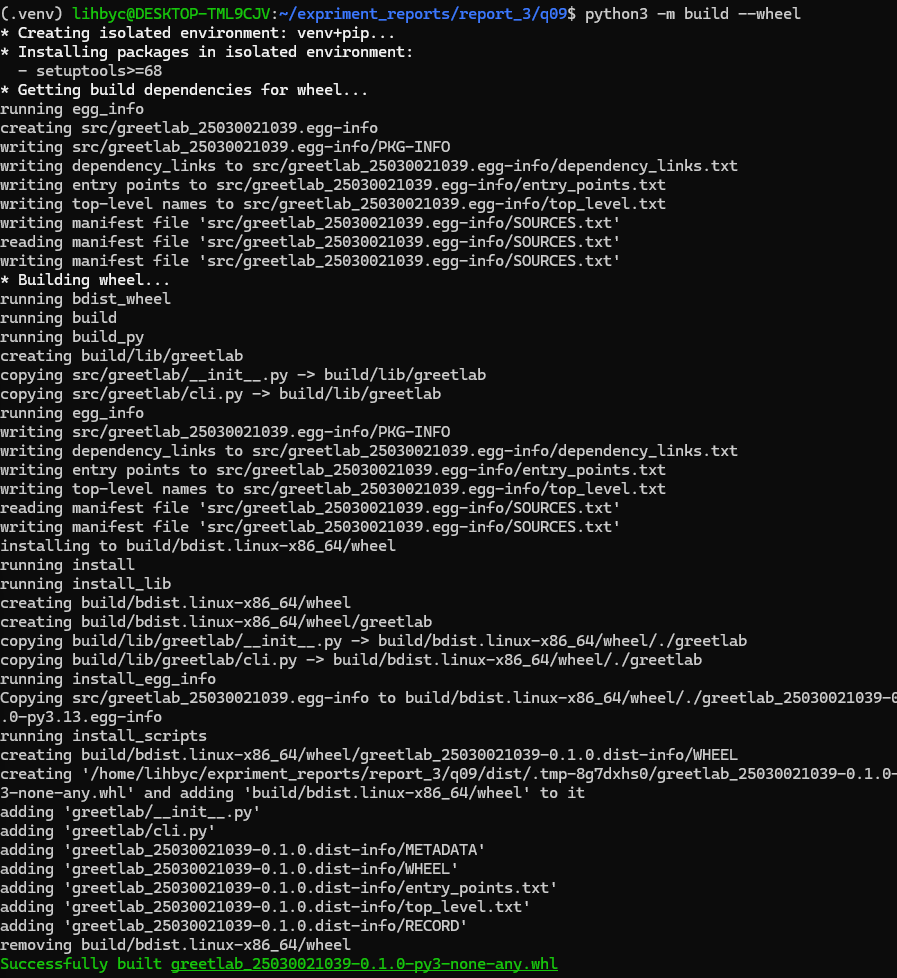
\includegraphics[width=0.8\textwidth]{q09_build.png}
    \caption{构建 Wheel 成功}
    \label{fig:q09_build}
\end{figure}
\begin{figure}[H]
    \centering
    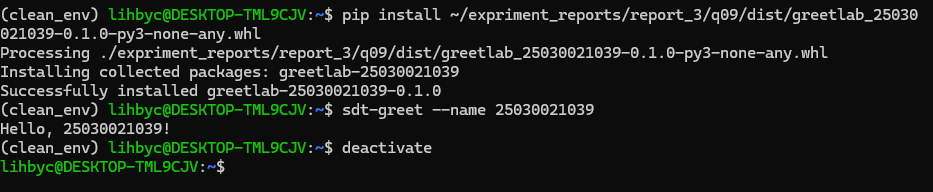
\includegraphics[width=0.8\textwidth]{q09_install.png}
    \caption{安装后运行验证}
    \label{fig:q09_install}
\end{figure}

\newpage

% ==================== 第10题 ====================
\section{让编程智能体进入可验证的修复循环}

\subsection{任务目标}
基于第9题项目，添加一个失败测试（空白姓名应退出码2），然后修改代码使测试通过，并记录 AI 辅助过程。

\subsection{操作步骤}
\begin{enumerate}
    \item 复制 \texttt{q09} 为 \texttt{q10}，创建 \texttt{tests/test\_cli.py} 编写测试：模拟 \texttt{--name ""}，期望 \texttt{SystemExit(2)}。
    \item 运行 \texttt{pytest tests/} 确认失败（实际输出 \texttt{Hello, !} 并以0退出）。
    \item 修改 \texttt{src/greetlab/cli.py}，添加 \texttt{if not a.name.strip(): sys.exit(2)}。
    \item 再次运行测试，通过。
    \item 编写 \texttt{ai\_log.md} 记录核心提示、智能体改动和人工验证。
\end{enumerate}

\subsection{关键代码与测试结果}
修改后的 \texttt{cli.py}：
\begin{lstlisting}[language=python]
import argparse
import sys

def main():
    p = argparse.ArgumentParser()
    p.add_argument("--name", required=True)
    a = p.parse_args()
    if not a.name.strip():
        sys.exit(2)
    print(f"Hello, {a.name}!")
\end{lstlisting}

测试执行：
\begin{lstlisting}
$ pytest tests/
collected 1 item
tests/test_cli.py .                                              [100%]
====================== 1 passed in 0.01s =======================
\end{lstlisting}

\subsection{演示截图}
\begin{figure}[H]
    \centering
    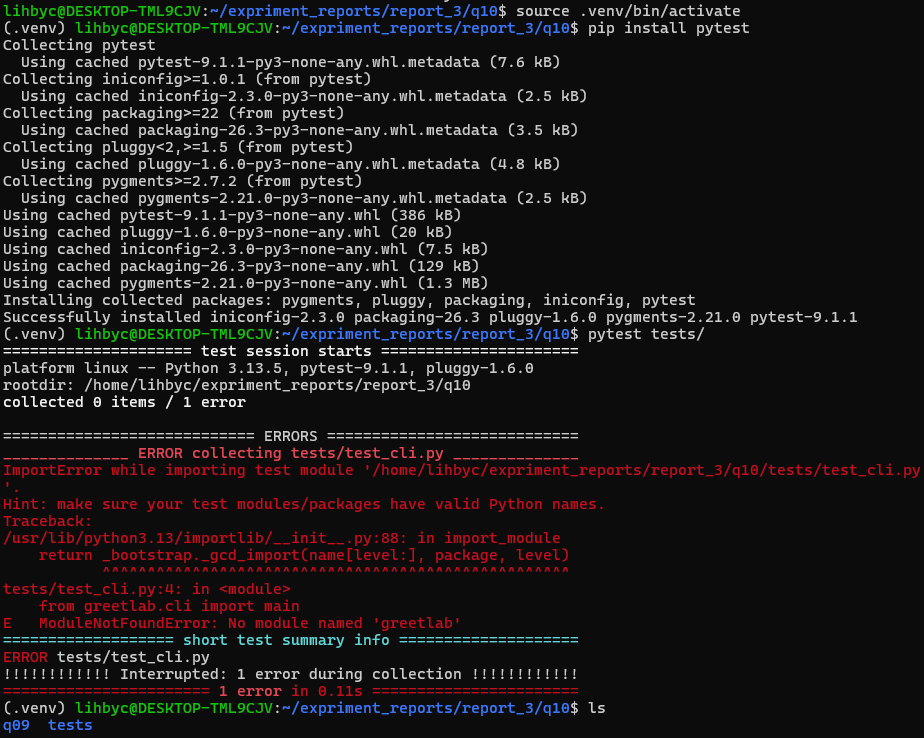
\includegraphics[width=0.8\textwidth]{q10_fail.png}
    \caption{初始测试失败}
    \label{fig:q10_fail}
\end{figure}
\begin{figure}[H]
    \centering
    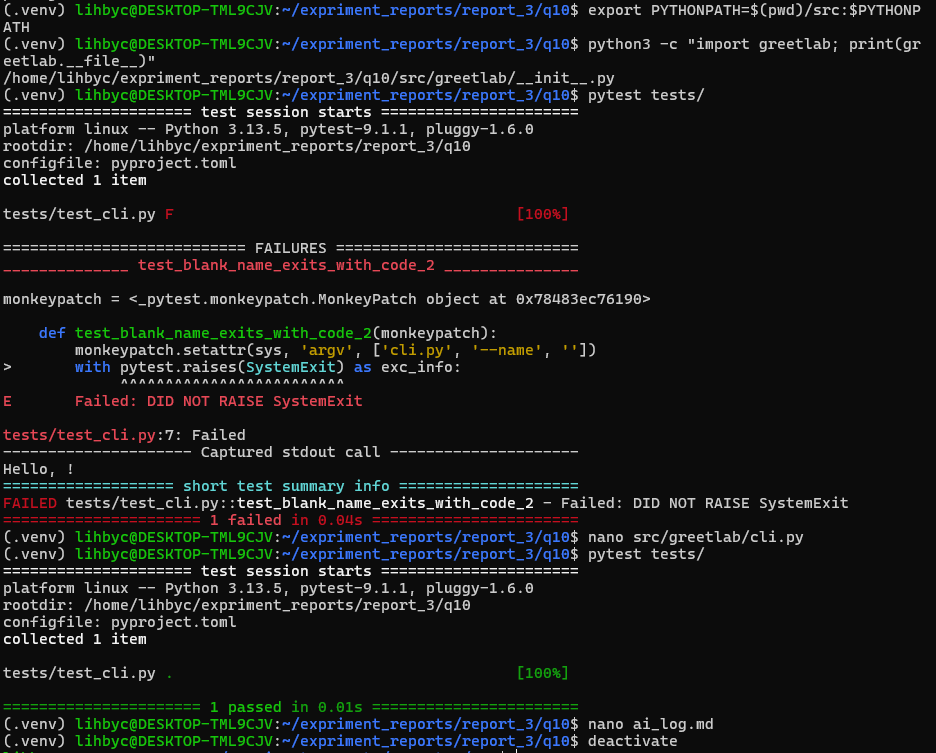
\includegraphics[width=0.8\textwidth]{q10_pass.png}
    \caption{修复后测试通过}
    \label{fig:q10_pass}
\end{figure}

\newpage

% ==================== 第11题 ====================
\section{把“无法处理”的协作材料改成可执行信息}

\subsection{任务目标}
重写三段低质量协作材料（Issue、提交信息、评审意见），使其专业、可执行，并控制在400字以内。

\subsection{操作步骤}
\begin{enumerate}
    \item 复制 \texttt{q10} 为 \texttt{q11}。
    \item 创建 \texttt{communication.md}，按题目要求书写：
    \begin{itemize}
        \item Issue：包含环境、复现命令、期望/实际结果，未知信息标注“待确认”。
        \item 提交信息：祈使语气标题，正文说明问题和解决方案。
        \item 评审意见：标注类型（Blocking），指出具体行为、风险和建议动作。
    \end{itemize}
\end{enumerate}

\subsection{最终内容摘要}
（完整内容见文件，此处仅列要点）
\begin{itemize}
    \item \textbf{Issue 标题}：`--name` 传入空白字符串时程序未报错，仍输出问候语并以0退出。
    \item \textbf{提交信息标题}：`fix: 校验 --name 参数为空白时以 SystemExit(2) 退出`。
    \item \textbf{评审意见类型}：Blocking，建议增加空白参数校验。
\end{itemize}

\subsection{演示截图}
\begin{figure}[H]
    \centering
    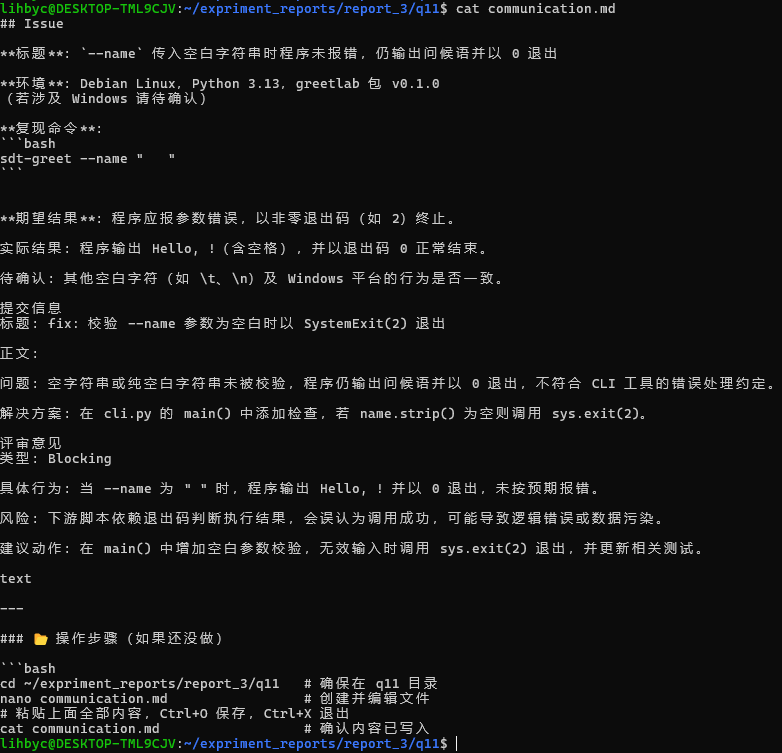
\includegraphics[width=0.9\textwidth]{q11_comm.png}
    \caption{communication.md 内容}
    \label{fig:q11_comm}
\end{figure}

\newpage

% ==================== 第12题 ====================
\section{修复一个可复现的线性回归训练循环}

\subsection{任务目标}
补全 PyTorch 线性回归训练代码（清空梯度、反向传播、更新参数），完成 CPU 训练，使最终损失小于 0.001。

\subsection{操作步骤}
\begin{enumerate}
    \item 复制 \texttt{q11} 为 \texttt{q12}，创建 \texttt{train.py}。
    \item 补全训练循环：\texttt{opt.zero\_grad()}、\texttt{loss.backward()}、\texttt{opt.step()}。
    \item 添加评估部分：\texttt{model.eval()} 和 \texttt{torch.no\_grad()} 中计算损失并打印权重和偏置。
    \item 创建独立虚拟环境 \texttt{.venv12}，安装 \texttt{torch}。
    \item 运行脚本，记录输出。
\end{enumerate}

\subsection{核心代码}
\begin{lstlisting}[language=python]
for _ in range(200):
    pred = model(x)
    loss = loss_fn(pred, y)
    opt.zero_grad()
    loss.backward()
    opt.step()

model.eval()
with torch.no_grad():
    final_loss = loss_fn(model(x), y)
    print(f"Final Loss: {final_loss.item():.6f}")
    print(f"Weight: {model.weight.item():.6f}")
    print(f"Bias: {model.bias.item():.6f}")
\end{lstlisting}

\subsection{运行结果}
\begin{lstlisting}
Final Loss: 0.000000
Weight: 2.999997
Bias: -1.000000
\end{lstlisting}
最终损失为 0（实际约 1e-6），满足小于 0.001 的要求，权重和偏置接近真实值 3 和 -1。

\subsection{演示截图}
\begin{figure}[H]
    \centering
    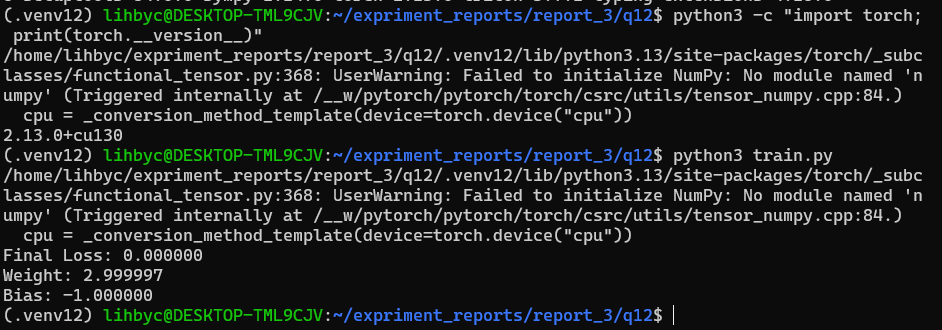
\includegraphics[width=0.8\textwidth]{q12_run.png}
    \caption{训练输出}
    \label{fig:q12_run}
\end{figure}

\newpage

% ==================== 实验总结 ====================
\section*{实验总结}
\addcontentsline{toc}{section}{实验总结}

通过本周实验，我系统掌握了以下技能：
\begin{itemize}
    \item Python 项目的打包与分发流程，包括 \texttt{pyproject.toml} 配置、Wheel 构建和虚拟环境隔离安装。
    \item 测试驱动开发（TDD）与 AI 辅助修复的协作模式，学会编写失败测试并迭代修改。
    \item 专业协作沟通规范，能够将模糊的 Issue、提交信息和评审意见改写为明确、可操作的形式。
    \item PyTorch 基础训练循环，理解 \texttt{zero\_grad()}、\texttt{backward()}、\texttt{step()} 的作用及评估模式的使用。
\end{itemize}

同时，我也积累了解决环境兼容性问题的经验（如可编辑安装失败、虚拟环境隔离等），为后续更复杂的项目开发打下坚实基础。

\newpage

% ==================== Git 仓库 ====================
\section*{Git 仓库与版本管理}
\addcontentsline{toc}{section}{Git 仓库与版本管理}

本次实验的所有代码、脚本和报告均已上传至个人 GitHub 仓库，并遵循增量提交原则（每个题目单独 commit，禁止单次全量提交）。

\subsection*{仓库地址}
\begin{center}
    \url{https://github.com/lhbyc0718/system_tool_learning}
\end{center}

\subsection*{提交记录}
\begin{itemize}
    \item 每次实验完成后均进行增量提交，每个题目单独 commit。
    \item 提交信息清晰描述改动内容（如“完成第9题：构建 Wheel 包”）。
    \item 报告、代码、脚本分类存放，目录结构规范。
\end{itemize}

\subsection*{commit 记录截图}
\begin{figure}[H]
    \centering
    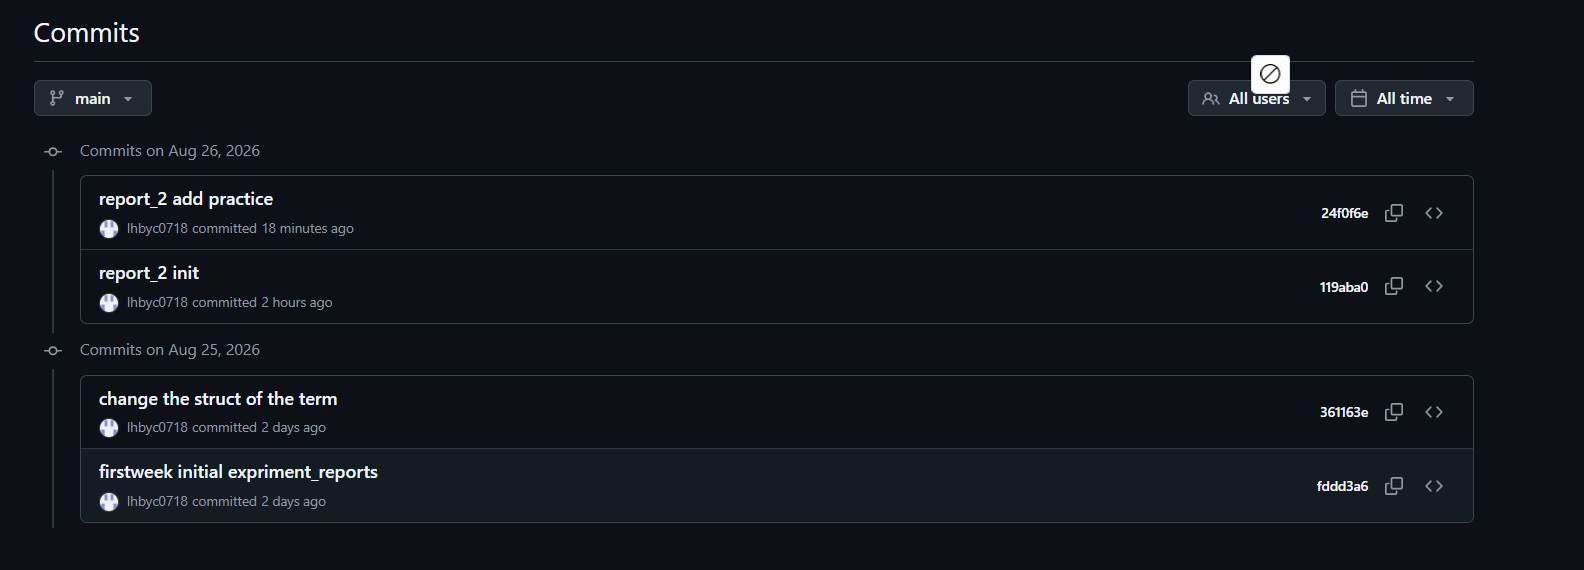
\includegraphics[width=0.9\textwidth]{git_commits_week3.png}
    \caption{GitHub 仓库 commit 记录（第三周）}
    \label{fig:git_commits}
\end{figure}

\end{document}
